\documentclass{protokol}
\leftheader{Studium ohybových jevů v laserovém svazku}
\centerheader{}
\rightheader{Tomáš Derner}

\begin{document}

  \section*{Úkol}

    \begin{enumerate}
      \item Ze změřeného ohybového obrazce zobrazeného na milimetrovém papíru určete mřížkovou konstantu mřížky.
      \item Pomocí aparatury proměřte ohybové obrazce: mřížky, štěrbiny a dvojštěrbiny. Konkrétní difrakční prvky vybere vyučující. Zpracováním měření určete parametry použitých difrakčních prvků.
      \item Okalibrujte mikroskopový okulár s použitím metody lineární regrese, odhadněte relativní chybu kalibrace.
      \item Mikroskopem změřte parametry všech použitých difrakčních prvků.
      \item Výsledky měření v úkolech č.1, č.2 a č.4 srovnejte a diskutujte, v kterém případě jsou spočtené parametry zatíženy nejmenší chybou. 
    \end{enumerate}

  \section*{Teorie}

    V tomto praktiku měříme ohyb laserového svazku způsobený difrakční mřížkou a štěrbinami. Protože použitý laser má poměrně velkou divergenci svazku, použijeme v měření spojnou čočku, viz \cite{mereni}. 

    Pro získání mřížkové konstanty $a$ využijeme vztahu pro úhel $\varphi$ mezi dvěma body maximální intenzity difrakčního obrazce
    \begin{equation} \label{eq:mrizkova_konstanta}
      \varphi = \frac{\lambda}{a},
    \end{equation} 
    kde $\lambda$ je vlnová délka použitého světla. Úhel $\varphi$ získáme z rovnice
    \begin{equation} \label{eq:phi}
      \varphi = \frac{x}{l},
    \end{equation}
    kde $x$ je vzdálenost dvou maxim a $l$ vzdálenost difrakčního obrazce od spojné čočky. Předpokládáme malé úhly.

  \section*{Výsledky}

    Vzdálenost difrakčních obrazců od čočky byla 
    $$ l = \SI{1.000 \pm 0.005}{m}. $$

    \subsection*{Úkol 1}

    \subsection*{Úkol 2}

      Intenzita světla vynesená v grafech níže nabývá hodnot 0 - 255 a popisuje odezvu snímače na dopadající světlo.

      V grafu \ref{fig:mrizka} je zobrazen difrakční obrazec difrakční mřížky. Odečtením poloh peaků a použitím vzorce \eqref{eq:mrizkova_konstanta} a \eqref{eq:phi} jsme dostali mřížkovou konstantu 
      $$ a = \SI{5.20 \pm 0.05 e-5}{m}. $$

      \begin{figure}[H]
        \centering
        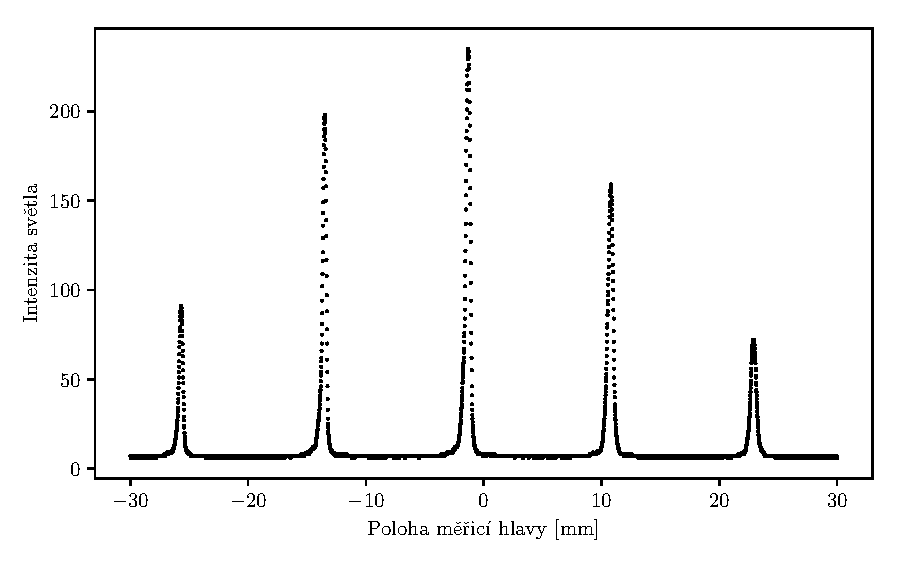
\includegraphics[]{mrizka} 
        \caption{Difrakční obrazec mřížky}
        \label{fig:mrizka}
      \end{figure}

    \subsection*{Úkol 3}

      Byla provedena kalibrace měřítka mikroskopu metodou postupných měření. Data byla zpracována lineární regresí, směrnice regrese je $\num{6.10 \pm 0.01}$. Jeden dílek na stupnici mikroskopu tedy odpovídá $\frac{1}{\num{6.10}}$ milimetrům.

    \subsection*{Úkol 4}

      Pomocí mikroskopu jsme získali rozměry použitých optických prvků, tabulka \ref{tab:mrizka} obsahuje vzdálenosti deseti vrypů mřížky, tabulka \ref{tab:sterbina_stredni} šířku štěrbiny na třech místech a tabulka \ref{tab:dvojs_blizke} šířku a vzdálenost štěrbin na třech místech.

      \begin{table}[H]
        \centering
        \setlength{\tabcolsep}{10pt}
        \begin{tabular}[t]{
  S[table-format=1.2]
  S[table-format=1.2]
  S[table-format=1.2e1]
} \toprule
{poloha vrypu}       & {vzdálenost od dalšího vrypu} & {vzdálenost od dalšího vrypu} \\
{[dílek mikroskopu]} & {[dílek mikroskopu]}          & {[m]}                         \\\midrule
3.54                 & 0.32                          & 5.24e-5                       \\
3.83                 & 0.29                          & 4.75e-5                       \\
4.16                 & 0.31                          & 5.08e-5                       \\
4.47                 & 0.32                          & 5.24e-5                       \\
4.79                 & 0.31                          & 5.08e-5                       \\
5.10                 & 0.32                          & 5.24e-5                       \\
5.42                 & 0.31                          & 5.08e-5                       \\
5.73                 & 0.33                          & 5.40e-5                       \\
6.02                 & 0.29                          & 4.75e-5                       \\
6.34                 &                               &                               \\\bottomrule
\end{tabular}

        \caption{Hodnoty vzdáleností vrypů mřížky}
        \label{tab:mrizka}
      \end{table}

      Průměrná hodnota vzdálenosti dvou vrypů a tedy i mřížkové konstanty je $$ a = \SI{5.09 \pm 0.07 e-5}{m}$$.
      
      \begin{table}[H]
        \centering
        \setlength{\tabcolsep}{5pt}
        \begin{tabular}[t]{
  S[table-format = 1.0]
  S[table-format = 1.2]
  S[table-format = 1.2]
  S[table-format = 1.2]
  S[table-format = 1.2e1]
} \toprule
{měření} & {poloha začátku št.} & {poloha konce št.} & {šířka štěrbiny}     & {šířka štěrbiny} \\
         & {[dílek mikroskopu]}      & {[dílek mikroskopu]}    & {[dílek mikroskopu]} & {[m]}            \\\midrule
1        & 2.50                      & 3.80                    & 1.30                 & 2.13e-4          \\
2        & 2.52                      & 3.81                    & 1.29                 & 2.11e-4          \\
3        & 2.74                      & 2.74                    & 1.24                 & 2.03e-4          \\\bottomrule
\end{tabular}

        \caption{Hodnoty šířky štěrbiny na třech místech}
        \label{tab:sterbina_stredni}
      \end{table}

      Průměrná hodnota šířky štěrbiny je $$ b = \SI{2.09 \pm 0.03 e-4}{m}$$.
      
      \begin{table}[H]
        \centering
        \setlength{\tabcolsep}{10pt}
        \begin{tabular}[t]{
  l
  S[table-format=1.3]
  S[table-format=1.3]
  S[table-format=1.3]
} \toprule
měření                         & {1}   & {2}   & {3}   \\\midrule
začátek první štěrbiny [dílek] & 2.08  & 2.20  & 2.06  \\
konec první štěrbiny [dílek]   & 2.75  & 2.94  & 2.80  \\\midrule
začátek druhé štěrbiny [dílek] & 5.72  & 5.90  & 5.76  \\
konec druhé štěrbiny [dílek]   & 6.46  & 6.75  & 6.51  \\\midrule
šířka první štěrbiny [dílek]   & 0.67  & 0.74  & 0.74  \\
šířka první štěrbiny [mm]      & 0.109 & 0.121 & 0.121 \\\midrule
šířka druhé štěrbiny [dílek]   & 0.74  & 0.85  & 0.75  \\
šířka druhé štěrbiny [mm]      & 0.121 & 0.140 & 0.123 \\\midrule
vzdálenost štěrbin [dílek]     & 3.64  & 3.70  & 3.70  \\
vzdálenost štěrbin [mm]        & 0.596 & 0.606 & 0.606 \\\bottomrule
\end{tabular}

        \caption{Hodnoty šířky a vzdálenosti štěrbin na třech místech}
        \label{tab:dvojs_blizke}
      \end{table}

      Aritmetický průměr vzdálenosti štěrbin je 
      $$ a = \SI{6.02 \pm 0.03 e-4}{m}. $$


  \section*{Diskuse}

  \section*{Závěr}

  \begin{thebibliography}{}

    \bibitem{mereni}
    Pokyny k měření "", dostupné z\\ \url{}, .\,.\,
  
  \end{thebibliography}

\end{document}